\section{Auswertung}
\label{sec:Auswertung}

\subsection{Die Charakteristik des Zählrohrs}

Die Messwerte der Impulszahlen $N$ über das Zeitintervall
von $t = \SI{125}{\second}$ in Abhängigkeit von der Spannung $U$, 
sowie die Impulsrate $\frac{N}{\SI{1}{\second}}$, deren Fehler
$\frac{\sqrt{N}}{t}$ und die Stromstärke $A$ sind in Tabelle \ref{tab:mess} abgebildet.

\begin{table}
  \centering
  \caption{Die Messdaten der Charakteristik des Zählrohrs in Abhängigkeit 
            von der angelegten Spannung $U$}
  \label{tab:mess}
  \sisetup{table-format=2.1}
  \begin{tabular}{c c c c c}
  \toprule
  $U \,/\, \si{\volt}$ & $N \text{ in } \SI{125}{\second}$ & 
  $\frac{N}{t} \;/\; \si{\per\second}$
  & $\frac{\sqrt{N}}{t} \;/\; \si{\per\second}$ & $A \,/\, \si{\micro\ampere}$\\
  \midrule 
  320 & 10726 & 85,81 & 0,83 & 0,20 \\
  340 & 10899 & 87,19 & 0,84 &  - \\
  360 & 11235 & 89,88 & 0,85 &  - \\
  380 & 11032 & 88,26 & 0,84 &  - \\
  400 & 11311 & 90,49 & 0,85 & 0,20 \\
  420 & 11211 & 89,69 & 0.85 &  - \\
  440 & 11216 & 89,73 & 0,85 &  - \\
  460 & 11055 & 88,44 & 0,84 &  - \\
  480 & 11235 & 89,88 & 0,85 & 0,25 \\
  500 & 11562 & 92,50 & 0,86 &  - \\
  520 & 11193 & 89,54 & 0,85 &  - \\
  540 & 11179 & 89,43 & 0,85 &  - \\
  560 & 11305 & 90,44 & 0,85 & 0,40 \\
  580 & 11269 & 90,15 & 0,85 &  - \\
  600 & 11314 & 90,51 & 0,85 &  - \\
  620 & 11462 & 91,70 & 0,86 &  - \\
  640 & 11559 & 92,47 & 0,86 & 0,50 \\
  660 & 11379 & 91,03 & 0,85 &  -  \\
  680 & 11830 & 94,64 & 0,87 & 0,50 \\
  \bottomrule
  \end{tabular}
  \end{table}

  In Abbildung \ref{fig:plot} ist die Impulsrate $\frac{N}{t}$ 
  gegen die Spannung $U$ aufgetragen. Es wird eine lineare Regression im 
  Plateauintervall von $\SI{400}{\volt}$ bis $\SI{600}{\volt}$  mittels
  Python mit der Geradengleichung $\frac{N}{t} = a \cdot U + b$ durchgeführt.
  Die Regressionsparameter ergeben sich dabei zu

  \begin{align*}
    a &= \SI{3.0 +- 5.6}{\per\second\per\kilo\per\volt} = \SI{0.33}{\percent\per100\volt}  \\
    b &= \SI{88.76 +- 2.83}{\per\second}   \;.
  \end{align*}

  Die Plateaulänge beträgt daher etwa $\SI{200}{\volt}$.

\begin{figure}
  \centering
  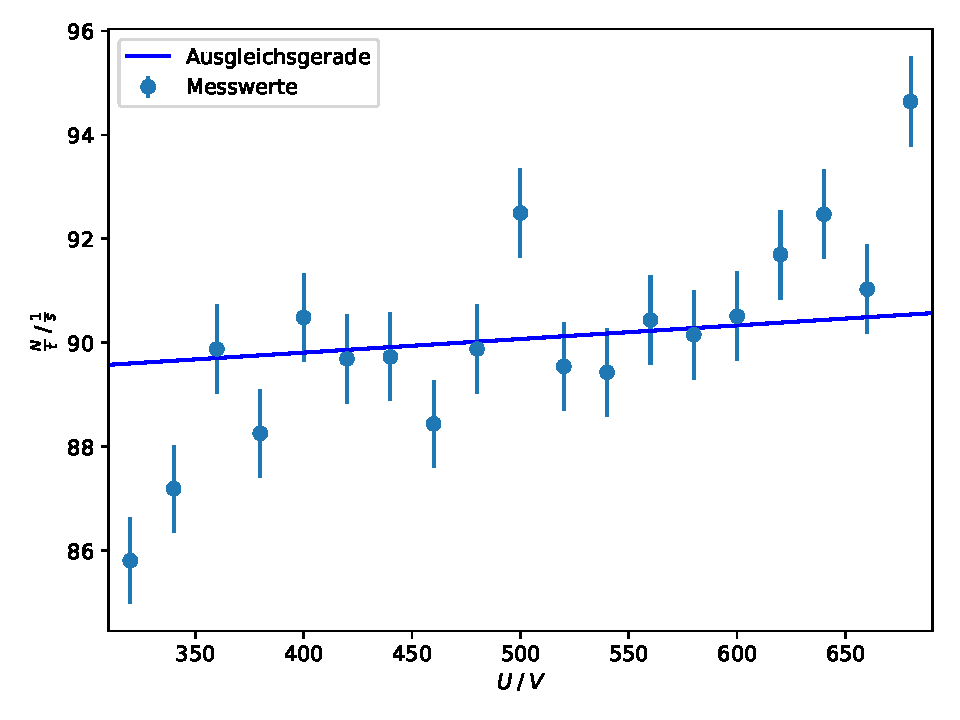
\includegraphics{content/plot1.pdf}
  \caption{Die spannungsabhängige Impulsrate}
  \label{fig:plot}
\end{figure}

\subsection{Nachentladungen des Zählrohrs}

Auf dem Oszilloskop konnte ein Abstand von $\SI{175}{\micro\second}$
zwischen Primär- und Nachentladung abgelesen werden.

\subsection{Die Totzeit des Zählrohrs}

Die nach der ersten Methode vom Oszilloskop abgelesene Totzeit betägt 
$\SI{30}{\micro\second}$. 

Durch die Zwei-Quellen-Methode über einen Zeitraum von
$t_\text{T} = \SI{100}{\second}$ ergeben sich für die Quellen 1 und 2
die Impulszahlen, die in Tabelle \ref{tab:mess2} aufgelistet sind.

\begin{table}
  \centering
  \caption{Die Messdaten zur Bestimmung der Totzeit des Zählrohrs}
\label{tab:mess2}
  \sisetup{table-format=2.1}
  \begin{tabular}{c c c c}
  \toprule
  Quelle & $N \text{ in } \SI{100}{\second}$ & 
  $\frac{N}{t} \;/\; \si{\per\second}$
  & $\frac{\sqrt{N}}{t} \;/\; \si{\per\second}$\\
  \midrule
  1     & 23514 & 235,14 & 1,53 \\
  2     & 35081 & 350,81 & 1,87 \\
  1 + 2 & 56651 & 566,51 & 2,38 \\
  \bottomrule
  \end{tabular}
  \end{table}

  Nach Gleichung \eqref{eqn:totzeit} ergibt sich die Totzeit zu 
  \begin{equation*}
   T_\text{T} = \SI{118 +- 20}{\micro\second} \;.
  \end{equation*}

  Der Fehler berechnet sich nach der Gaußschen Fehlerfortpflanzung gemäß

  \begin{equation}
    \symup{\Delta} T_\text{T} = \frac{n_{1+2} - n_2}{2 n_1^2 n_2} \cdot \symup{\Delta} n_1
    + \frac{n_{1+2} - n_1}{2 n_2^2 n_1} \symup{\Delta} n_1 -
    \frac{1}{2 n_1 n_2} \symup{\Delta} n_{1+2} \; .
  \end{equation}




